%%%%%%%%%%%%%%%%%%%%%%%%%%%%%%%%%%%%%%%%%
% Beamer Presentation
% LaTeX Template
% Version 1.0 (10/11/12)
%
% This template has been downloaded from:
% http://www.LaTeXTemplates.com
%
% License:
% CC BY-NC-SA 3.0 (http://creativecommons.org/licenses/by-nc-sa/3.0/)
%
%%%%%%%%%%%%%%%%%%%%%%%%%%%%%%%%%%%%%%%%%

%----------------------------------------------------------------------------------------
%	PACKAGES AND THEMES
%----------------------------------------------------------------------------------------

\documentclass[handout]{beamer}

\mode<presentation> {

% The Beamer class comes with a number of default slide themes
% which change the colors and layouts of slides. Below this is a list
% of all the themes, uncomment each in turn to see what they look like.

%\usetheme{default}
%\usetheme{AnnArbor}
%\usetheme{Antibes}
%\usetheme{Bergen}
%\usetheme{Berkeley}
%\usetheme{Berlin}
%\usetheme{Boadilla}
%\usetheme{CambridgeUS}
%\usetheme{Copenhagen}
%\usetheme{Darmstadt}
%\usetheme{Dresden}
%\usetheme{Frankfurt}
%\usetheme{Goettingen}
%\usetheme{Hannover}
%\usetheme{Ilmenau}
%\usetheme{JuanLesPins}
%\usetheme{Luebeck}
\usetheme{Madrid}
%\usetheme{Malmoe}
%\usetheme{Marburg}
%\usetheme{Montpellier}
%\usetheme{PaloAlto}
%\usetheme{Pittsburgh}
%\usetheme{Rochester}
%\usetheme{Singapore}
%\usetheme{Szeged}
%\usetheme{Warsaw}

% As well as themes, the Beamer class has a number of color themes
% for any slide theme. Uncomment each of these in turn to see how it
% changes the colors of your current slide theme.

%\usecolortheme{albatross}
%\usecolortheme{beaver}
%\usecolortheme{beetle}
%\usecolortheme{crane}
%\usecolortheme{dolphin}
%\usecolortheme{dove}
%\usecolortheme{fly}
%\usecolortheme{lily}
%\usecolortheme{orchid}
%\usecolortheme{rose}
%\usecolortheme{seagull}
%\usecolortheme{seahorse}
%\usecolortheme{whale}
%\usecolortheme{wolverine}

%\setbeamertemplate{footline} % To remove the footer line in all slides uncomment this line
%\setbeamertemplate{footline}[page number] % To replace the footer line in all slides with a simple slide count uncomment this line

%\setbeamertemplate{navigation symbols}{} % To remove the navigation symbols from the bottom of all slides uncomment this line
}

\usepackage{graphicx} % Allows including images
\usepackage{booktabs} % Allows the use of \toprule, \midrule and \bottomrule in tables
\usepackage{cool}
\usepackage{amsmath}
\usepackage{amssymb}
\usepackage{bm}
\usepackage{physics}
\usepackage{hyperref}
\usepackage{listings}
\usepackage{enumerate}

\newcommand{\prob}{\mathcal{P}}
\newcommand{\rew}{\mathcal{R}}
\newcommand{\states}{\mathcal{S}}
\newcommand{\actions}{\mathcal{S}}

\DeclareMathOperator*{\argmin}{arg\,min}
\DeclareMathOperator*{\argmax}{arg\,max}

\newcommand{\bvpi}{\bm{V}^{\pi}}
\newcommand{\bvs}{\bm{V}^*}
\newcommand{\bbpi}{\bm{B}^{\pi}}
\newcommand{\bbs}{\bm{B}^*}
\newcommand{\bv}{\bm{V}}

%----------------------------------------------------------------------------------------
%	TITLE PAGE
%----------------------------------------------------------------------------------------

\title[Dynamic Programming Chapter]{A Guided Tour of \href{http://stanford.edu/~ashlearn/RLForFinanceBook/book.pdf}{\underline{\textcolor{yellow}{Chapter 3}}}: \\  Dynamic Programming} % The short title appears at the bottom of every slide, the full title is only on the title page

\author{Ashwin Rao} % Your name
\institute[Stanford] % Your institution as it will appear on the bottom of every slide, may be shorthand to save space
{ICME, Stanford University
 % Your institution for the title page
}

\date % Date, can be changed to a custom date

\begin{document}
\lstset{language=Python}  
\begin{frame}
\titlepage % Print the title page as the first slide
\end{frame}

% \begin{frame}
% \frametitle{Overview} % Table of contents slide, comment this block out to remove it
% \tableofcontents % Throughout your presentation, if you choose to use \section{} and \subsection{} commands, these will automatically be printed on this slide as an overview of your presentation
% \end{frame}

\begin{frame}
\frametitle{Dynamic Programming for Prediction and Control}
\pause
\begin{itemize}[<+->]
\item Prediction: Compute the Value Function of an MRP
\item Control: Compute the Optimal Value Function of an MDP
\item (Optimal Policy can be extracted from Optimal Value Function)
\item Planning versus Learning: access to the $\mathcal{P}_R$ function (``model'')
\item Original use of {\em DP} term: MDP Theory {\em and} solution methods
\item Bellman refered to DP as the {\em Principle of Optimality}
\item Later, the usage of the term DP diffused out to other algorithms
\item In CS, it means "recursive algorithms with overlapping subproblems"
\item We restrict the term DP to: "Algorithms for Prediction and Control"
\item Specifically applied to the setting of \lstinline{FiniteMarkovDecisionProcess}
\item Later we cover extensions such as Asynchronous DP, Approximate DP
\end{itemize}
\end{frame}

\begin{frame}
\frametitle{Solving the Value Function as a {\em Fixed-Point}}
\pause
\begin{itemize}[<+->]
\item We will be covering 3 Dynamic Programming algorithms
\item Each of the 3 algorithms is founded on the Bellman Equations
\item Each is an iterative algorithm converging to the true Value Function
\item Each algorithm is based on the concept of {\em Fixed-Point}
\begin{definition}
The Fixed-Point of a function $f: \mathcal{X} \rightarrow \mathcal{X}$ (for some arbitrary domain $\mathcal{X}$) is a value $x \in \mathcal{X}$ that satisfies the equation: $x = f(x)$.
\end{definition}
\item Some functions have multiple fixed-points, some have none
\item DP algorithms are based on functions with a unique fixed-point
\item Simple example: $f(x) = \cos(x)$, Fixed-Point:  $x^* = \cos(x^*)$
\item For any $x_0$, $\cos(\cos(\ldots \cos(x_0) \ldots))$ converges to fixed-point $x^*$
\item Why does this work? How fast does it converge? 
\end{itemize}
\end{frame}

\begin{frame}
\frametitle{Banach Fixed-Point Theorem}
\pause
\begin{theorem}[Banach Fixed-Point Theorem]
Let $\mathcal{X}$ be a non-empty set equipped with a complete metric $d: \mathcal{X} \times \mathcal{X} \rightarrow \mathbb{R}$. Let $f: \mathcal{X} \rightarrow \mathcal{X}$ be such that there exists a $L \in [0, 1)$ such that
$d(f(x_1), f(x_2)) \leq L \cdot d(x_1, x_2)$ for all $x_1, x_2 \in \mathcal{X}$. Then,
\pause
\begin{itemize}[<+->]
\item There exists a unique Fixed-Point $x^* \in \mathcal{X}$, i.e.,
$$x^* = f(x^*)$$
\item For any $x_0 \in \mathcal{X}$, and sequence $[x_i|i=0, 1, 2, \ldots]$ defined as $x_{i+1} = f(x_i)$ for all $i = 0, 1, 2, \ldots$,
$$\lim_{i\rightarrow \infty} x_i = x^*$$
\end{itemize}
\end{theorem}
\pause
If you have a complete metric space $\langle \mathcal{X}, d \rangle$ and a contraction $f$ (with respect to $d$), then you have an algorithm to solve for the fixed-point of $f$.
\end{frame}

\begin{frame}
\frametitle{{\em Policy Evaluation} (for {\em Prediction})}
\pause
\begin{itemize}[<+->]
\item MDP with $\mathcal{S} = \{s_1, s_2, \ldots, s_n\}, \mathcal{N} = \{s_1, s_2, \ldots, s_m \}$
\item Given a policy $\pi$, compute the Value Function of $\pi$-implied MRP
\item $\mathcal{P}_R^{\pi}: \mathcal{N} \times \mathcal{D} \times \mathcal{S} \rightarrow [0, 1]$ is given as a data structure
\item Extract (from $\mathcal{P}_R^{\pi}$) $\mathcal{P}^{\pi}: \mathcal{N} \times \mathcal{S} \rightarrow [0, 1]$ and  $\mathcal{R}^{\pi}: \mathcal{N} \rightarrow \mathbb{R}$
\item For non-large spaces, we can compute (in vector notation):
$${\bm V}^{\pi} = (\bm{I_m} - \gamma \bm{\mathcal{P}}^{\pi})^{-1} \cdot \bm{\mathcal{R}}^{\pi}$$
\item Note: $\bvpi, \bm{\mathcal{R}}^{\pi}$ are $m$-column vectors ($\in \mathbb{R}^m$) and $\bm{\mathcal{P}}^{\pi}$ is $m \times m$ matrix
\item So we look for an iterative algorithm to solve MRP Bellman Equation:
$$\bvpi  = \bm{\mathcal{R}}^{\pi} + \gamma \bm{\mathcal{P}}^{\pi} \cdot \bvpi$$
\end{itemize}
\end{frame}

\begin{frame}
\frametitle{Bellman Policy Operator and it's Fixed-Point}
\pause
\begin{itemize}[<+->]
\item Define the {\em Bellman Policy Operator} $\bbpi: \mathbb{R}^m \rightarrow \mathbb{R}^m$ as:
$$\bbpi(\bv) = \bm{\mathcal{R}}^{\pi} + \gamma \bm{\mathcal{P}}^{\pi} \cdot \bv \text{ for any Value Function vector } \bv \in \mathbb{R}^m$$
\item $\bbpi$ is a linear transformation on vectors in $\mathbb{R}^m$
\item So, the MRP Bellman Equation can be expressed as:
$$\bvpi = \bbpi(\bvpi)$$
\item This means $\bvpi \in \mathbb{R}^m$ is the Fixed-Point of $\bbpi: \mathbb{R}^m \rightarrow \mathbb{R}^m$
\item Metric $d: \mathbb{R}^m \times \mathbb{R}^m \rightarrow \mathbb{R}$ defined as $L^{\infty}$ norm:
$$d(\bm{X}, \bm{Y}) = \Vert \bm{X} - \bm{Y} \Vert_{\infty} = \max_{s \in \mathcal{N}} |(\bm{X} - \bm{Y})(s)|$$
\item $\bbpi$ is a contraction function under $L^{\infty}$ norm: For all $\bm{X}, \bm{Y} \in \mathbb{R}^m$,
$$\max_{s \in \mathcal{N}} |(\bbpi(\bm{X}) - \bbpi(\bm{Y}))(s)| = \gamma \cdot \max_{s \in \mathcal{N}} |(\bm{\mathcal{P}}^{\pi} \cdot (\bm{X} - \bm{Y}))(s)|$$
$$ \leq \gamma \cdot \max_{s \in \mathcal{N}} |(\bm{X} - \bm{Y})(s)|$$
\end{itemize}
\end{frame}

\begin{frame}
\frametitle{Policy Evaluation Convergence Theorem}
Invoking the Banach Fixed-Point Theorem for $\gamma < 1$ gives:
\pause
\begin{theorem}[Policy Evaluation Convergence Theorem]
For a Finite MDP with $|\mathcal{N}| = m$ and $\gamma < 1$, if $\bvpi \in \mathbb{R}^m$ is the Value Function of the MDP when evaluated with a fixed policy $\pi: \mathcal{N} \times \mathcal{A} \rightarrow [0, 1]$, then $\bvpi$ is the unique Fixed-Point of the Bellman Policy Operator $\bbpi: \mathbb{R}^m \rightarrow \mathbb{R}^m$, and
$$\lim_{i\rightarrow \infty} ({\bbpi})^i(\bm{V_0}) \rightarrow \bvpi \text{ for all starting Value Functions } \bm{V_0} \in \mathbb{R}^m$$
\end{theorem}
\end{frame}

\begin{frame}
\frametitle{Policy Evaluation algorithm}
\pause
\begin{itemize}[<+->]
\item Start with any Value Function $\bm{V_0} \in \mathbb{R}^m$
\item Iterating over $i = 0, 1, 2, \ldots$, calculate in each iteration:
  $$\bm{V_{i+1}} = \bbpi(\bm{V_i}) = \bm{\mathcal{R}}^{\pi} + \gamma \bm{\mathcal{P}}^{\pi} \cdot \bm{V_i}$$
\item Stop when $d(\bm{V_i}, \bm{V_{i+1}}) = \max_{s \in \mathcal{N}} |(\bm{V_i} - \bm{V_{i+1}})(s)|$ is small enough
\end{itemize}
\vspace{5mm}
\pause
Banach Fixed-Point Theorem also assures speed of convergence (dependent on choice of starting Value Function $\bm{V_0}$ and on choice of $\gamma$).\\
\vspace{5mm}
\pause
Running time of each iteration is $O(m^2)$. Constructing the MRP from the MDP and the policy takes $O(m^2 k)$ operations, where $m = |\mathcal{N}|, k = |\mathcal{A}|$.

\end{frame}

\begin{frame}
\frametitle{Greedy Policy}
\pause
\begin{itemize}[<+->]
\item Now we move on solving the MDP {\em Control} problem
\item We want to iterate {\em Policy Improvements} to drive to an {\em Optimal Policy}
\item {\em Policy Improvement} is based on a ``greedy'' technique
\item The {\em Greedy Policy Function} $G: \mathbb{R}^m \rightarrow (\mathcal{N} \rightarrow \mathcal{A})$\\
(interpreted as a function mapping a Value Function vector $\bv$ to a deterministic policy $\pi_D': \mathcal{N} \rightarrow \mathcal{A}$) is defined as:
$$G(\bv)(s) = \pi_D'(s) = \argmax_{a\in \mathcal{A}} \{\mathcal{R}(s,a) + \gamma \sum_{s' \in \mathcal{N}} \mathcal{P}(s,a,s') \cdot \bv(s') \}$$
\end{itemize}
\pause
\begin{definition}[Value Function Comparison]
We say $X \geq Y$ for Value Functions $X, Y: \mathcal{N} \rightarrow \mathbb{R}$ of an MDP iff:
$$X(s) \geq Y(s) \text{ for all } s \in \mathcal{N}$$
\end{definition}
\pause
We say $\pi_1$ better (``improvement'') than $\pi_2$ if $\bm{V}^{\pi_1} \geq \bm{V}^{\pi_2}$
\end{frame}

\begin{frame}
\frametitle{Policy Improvement Theorem}
\begin{theorem}[Policy Improvement Theorem]
For a finite MDP, for any policy $\pi$,
$$\bm{V}^{\pi_D'} = \bm{V}^{G(\bvpi)} \geq \bvpi$$
\label{th:policy_improvement_theorem}
\end{theorem}
\pause
\begin{itemize}[<+->]
\item Note that applying $\bm{B}^{\pi_D'} = \bm{B}^{G(\bvpi)}$ repeatedly, starting with $\bvpi$, will converge to $\bm{V}^{\pi_D'}$ (Policy Evaluation with policy $\pi_D' = G(\bvpi)$):
$$\lim_{i\rightarrow \infty} (\bm{B}^{\pi_D'})^i(\bvpi) = \bm{V}^{\pi_D'}$$
\item So the proof is complete if we prove that:
$$(\bm{B}^{\pi_D'})^{i+1}(\bvpi) \geq (\bm{B}^{\pi_D'})^i(\bvpi) \text{ for all } i = 0, 1, 2, \ldots$$
\item Increasing tower of Value Functions $[(\bm{B}^{\pi_D'})^i(\bvpi)|i = 0, 1, 2, \ldots]$ with repeated applications of $\bm{B}^{\pi_D'}$
\end{itemize}
\end{frame}

\begin{frame}
\frametitle{Proof by Induction}
\pause
\begin{itemize}[<+->]
\item To prove the base case (of proof by induction), note that:
$$\bm{B}^{\pi_D'}(\bvpi)(s) = \max_{a \in \mathcal{A}} \{\mathcal{R}(s,a) + \gamma \sum_{s' \in \mathcal{N}} \mathcal{P}(s,a,s') \cdot \bvpi(s')\} = \max_{a \in \mathcal{A}} Q^{\pi}(s,a)$$
\item $\bvpi(s)$ is weighted average of $Q^{\pi}(s,\cdot)$ while $\bm{B}^{\pi_D'}(\bvpi)(s)$ is maximum
$$\bm{B}^{\pi_D'}(\bvpi) \geq \bvpi$$
\item Induction step is proved by monotonicity of $\bm{B}^{\pi}$ operator (for any $\pi$):
$$\text{Monotonicity Property of } \bm{B}^{\pi}: \bm{X} \geq \bm{Y} \Rightarrow \bm{B}^{\pi}(\bm{X}) \geq \bm{B}^{\pi}(\bm{Y})$$
$$\text{So } (\bm{B}^{\pi_D'})^{i+1}(\bvpi) \geq (\bm{B}^{\pi_D'})^i(\bvpi) \Rightarrow (\bm{B}^{\pi_D'})^{i+2}(\bvpi) \geq (\bm{B}^{\pi_D'})^{i+1}(\bvpi)$$
\end{itemize}
\end{frame}


\begin{frame}
\frametitle{Intuitive Understanding of Policy Improvement Theorem}
\pause
\begin{itemize}[<+->]	
\item Increasing tower of Value Functions $[(\bm{B}^{\pi_D'})^i(\bvpi)|i = 0, 1, 2, \ldots]$
\item Each stage of further application of $\bm{B}^{\pi_D'}$ improves the Value Function
\item Stage 0:  Value Function $\bvpi$ means execute policy $\pi$ throughout
\item Stage 1: VF $\bm{B}^{\pi_D'}(\bvpi)$ means execute improved policy $\pi_D'$ for the 1st time step, then execute policy $\pi$ for all further time steps
\item Improves the VF from Stage 0: $\bvpi$ to Stage 1: $\bm{B}^{\pi_D'}(\bvpi)$
\item Stage 2: VF $(\bm{B}^{\pi_D'})^2(\bvpi)$ means execute improved policy $\pi_D'$ for first 2 time steps, then execute policy $\pi$ for all further time steps
\item Improves the VF from Stage 1: $\bm{B}^{\pi_D'}(\bvpi)$ to Stage 2: $(\bm{B}^{\pi_D'})^2(\bvpi)$
\item Each stage applies policy $\pi_D'$ instead of $\pi$ for an extra time step
\item These stages are the iterations of {\em Policy Evaluation} (using policy $\pi_D'$)
\item Building an increasing tower of VFs that converge to VF $\bm{V}^{\pi_D'}$ ($\geq \bvpi$)
\end{itemize}
\end{frame}

\begin{frame}
\frametitle{Repeating Policy Improvement and Policy Evaluation}
\pause
\begin{itemize}[<+->]
\item Policy Improvement Theorem says:
\begin{itemize}[<+->]
\item Start with Value Function $\bvpi$ (for policy $\pi$)
\item Perform a ``greedy policy improvement'' to create policy $\pi_D' = G(\bvpi)$
\item Perform Policy Evaluation (for policy $\pi_D'$) with starting VF $\bvpi$
\item This results in VF $\bm{V}^{\pi_D'} \geq$ starting VF $\bvpi$
\end{itemize}
\item We can repeat this process starting with $\bm{V}^{\pi_D'}$
\item Creating an improved policy $\pi_D''$ and improved VF $\bm{V}^{\pi_D''}$.
\item ... and we can keep going to create further improved policies/VFs
\item ... until there is no further improvement
\item This in fact is the {\em Policy Iteration} algorithm
\end{itemize}
\end{frame}

\begin{frame}
\frametitle{Policy Iteration algorithm}
\pause
\begin{itemize}[<+->]
\item Start with any Value Function $\bm{V_0} \in \mathbb{R}^m$
\item Iterating over $j = 0, 1, 2, \ldots$, calculate in each iteration:
$$\text{ Deterministic Policy } \pi_{j+1} = G(\bm{V_j})$$
$$\text{ Value Function } \bm{V_{j+1}} = \lim_{i\rightarrow \infty} (\bm{B}^{\pi_{j+1}})^i(\bm{V_j})$$
\item Stop when $d(\bm{V_j}, \bm{V_{j+1}}) = \max_{s \in \mathcal{N}} |(\bm{V_j} - \bm{V_{j+1}})(s)|$ is small enough
\end{itemize}
\pause
$$\text{At termination: } \bm{V_j} = (\bm{B}^{G(\bm{V_j})})^i(\bm{V_j}) = \bm{V_{j+1}} \text{ for all } i = 0, 1, 2, \ldots$$
\pause
Specializing this to $i=1$, we have for all $s \in \mathcal{N}$:
$$\bm{V_j}(s) = \bm{B}^{G(\bm{V_j})}(\bm{V_j})(s) = \max_{a \in \mathcal{A}} \{\mathcal{R}(s,a) + \gamma \sum_{s' \in \mathcal{N}} \mathcal{P}(s,a,s') \cdot \bm{V_j}(s')\}$$
\pause
This means $\bm{V_j}$ satisfies the MDP Bellman Optimality Equation and so,
$$\bm{V_j} = \bm{V}^{\pi_j} = \bvs$$
\end{frame}

\begin{frame}
\frametitle{Policy Iteration algorithm}
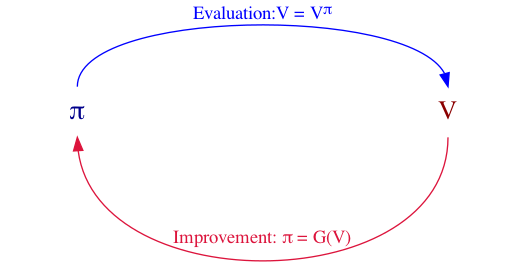
\includegraphics[width=12cm, height=5cm]{policy_iteration_loop.png}

\includegraphics[width=12cm, height=2cm]{policy_iteration_convergence.png}
\end{frame}

\begin{frame}
\frametitle{Policy Iteration Convergence Theorem}
\begin{theorem}[Policy Iteration Convergence Theorem]
For a Finite MDP with $|\mathcal{N}| = m$ and $\gamma < 1$, Policy Iteration algorithm converges to the Optimal Value Function $\bvs \in \mathbb{R}^m$ along with a Deterministic Optimal Policy $\pi_D^*: \mathcal{N} \rightarrow \mathcal{A}$, no matter which Value Function $\bm{V_0} \in \mathbb{R}^m$ we start the algorithm with.
\label{eq:policy_iteration_convergence_theorem}
\end{theorem}
\vspace{5mm}
\pause
Running time of Policy Improvement is $O(m^2 k)$ where $|\mathcal{N}| = m, |\mathcal{A}| = k$\\
\vspace{2mm}
\pause
Running time of each iteration of Policy Evaluation is $O(m^2 k)$
\end{frame}


\begin{frame}
\frametitle{Bellman Optimality Operator}
\pause
\begin{itemize}[<+->]
\item Tweak the definition of Greedy Policy Function ($\argmax$ to $\max$)
\item {\em Bellman Optimality Operator} $\bbs: \mathbb{R}^m \rightarrow \mathbb{R}^m$ defined as:
$$\bbs(\bv)(s) = \max_{a\in \mathcal{A}} \{\mathcal{R}(s,a) + \gamma \sum_{s' \in \mathcal{N}} \mathcal{P}(s,a,s') \cdot \bv(s')\}$$
\item Think of this as a non-linear transformation of a VF vector $\bv \in \mathbb{R}^m$
\item The action $a$ producing the max is the action prescribed by $\pi_D$. So,
$$\bm{B}^{G(\bv)}(\bv) = \bbs(\bv) \text{ for all } \bv \in \mathbb{R}^m$$
\item Specializing $\bv$ to be the Value Function $\bvpi$ for a policy $\pi$, we get:
$$\bm{B}^{G(\bvpi)}(\bvpi) = \bbs(\bvpi)$$
\item This is the 1st stage of Policy Evaluation with improved policy $G(\bvpi)$
\end{itemize}
\end{frame}

\begin{frame}
\frametitle{Fixed-Point of Bellman Optimality Operator}
\pause
\begin{itemize}[<+->]
\item $\bbpi$ was motivated by the MDP Bellman Policy Equation
\item Similarly, $\bbs$ is motivated by the MDP Bellman Optimality Equation:
$$\bvs(s) = \max_{a \in \mathcal{A}} \{ \mathcal{R}(s,a) + \gamma \sum_{s' \in \mathcal{N}} \mathcal{P}(s,a,s') \cdot \bvs(s') \} \text{ for all } s \in \mathcal{N}$$
\item So we can express the MDP Bellman Optimality Equation neatly as:
$$\bvs = \bbs(\bvs)$$
\item Therefore, $\bvs \in \mathbb{R}^m$ is the Fixed-Point of $\bbs: \mathbb{R}^m \rightarrow \mathbb{R}^m$
\item We want to prove that $\bbs$ is a contraction function (under $L^{\infty}$ norm)
\item So we can take advantage of Banach Fixed-Point Theorem
\item And solve the Control problem by iterative applications of $\bbs$
\end{itemize}
\end{frame}

\begin{frame}
\frametitle{Proof that $\bbs$ is a contraction}
\pause
\begin{itemize}[<+->]
\item We need to utilize two key properties of $\bbs$
$$\text{Monotonicity Property: } \bm{X} \geq \bm{Y} \Rightarrow \bbs(\bm{X}) \geq \bbs(\bm{Y})$$
$$ \text{Constant Shift Property: } \bbs(\bm{X} + c) = \bbs(\bm{X}) + \gamma c$$
\item With these two properties, we can prove that:
$$\max_{s \in \mathcal{N}} |(\bbs(\bm{X}) - \bbs(\bm{Y}))(s)| \leq \gamma \cdot \max_{s\in \mathcal{N}} |(\bm{X} - \bm{Y})(s)|$$
\end{itemize}
\pause
\begin{theorem}[Value Iteration Convergence Theorem]
For a Finite MDP with $|\mathcal{N}| = m$ and $\gamma < 1$, if $\bvs \in \mathbb{R}^m$ is the Optimal Value Function, then $\bvs$ is the unique Fixed-Point of the Bellman Optimality Operator $\bbs: \mathbb{R}^m \rightarrow \mathbb{R}^m$, and
$$\lim_{i\rightarrow \infty} (\bbs)^i(\bm{V_0}) \rightarrow \bvs \text{ for all starting Value Functions } \bm{V_0} \in \mathbb{R}^m$$
\label{eq:policy_evaluation_convergence_theorem}
\end{theorem}
\end{frame}

\begin{frame}
\frametitle{Value Iteration algorithm}
\pause
\begin{itemize}[<+->]
\item Start with any Value Function $\bm{V_0} \in \mathbb{R}^m$
\item Iterating over $i = 0, 1, 2, \ldots$, calculate in each iteration:
$$\bm{V_{i+1}}(s) = \bbs(\bm{V_i})(s) \text{ for all } s \in \mathcal{N}$$
\item Stop when $d(\bm{V_i}, \bm{V_{i+1}}) = \max_{s \in \mathcal{N}} |(\bm{V_i} - \bm{V_{i+1}})(s)|$ is small enough
\end{itemize}
\pause
\vspace{5mm}
Running time of each iteration of Value Iteration is $O(m^2 k)$ where $|\mathcal{N}| = m$ and $|\mathcal{A}| = k$
\end{frame}

\begin{frame}
\frametitle{Optimal Policy from Optimal Value Function}
\pause
\begin{itemize}[<+->]
\item Note that Value Iteration does not deal with any policy (only VFs)
\item Extract Optimal Policy $\pi^*$ from Optimal VF $V^*$ such that $\bm{V}^{\pi^*} = \bvs$
\item Use Greedy Policy function $G$. We know:
$$\bm{B}^{G(\bv)}(\bv) = \bbs(\bv) \text{ for all } \bv \in \mathbb{R}^m$$
\item Specializing $\bv$ to $\bvs$, we get:
$$\bm{B}^{G(\bvs)}(\bvs) = \bbs(\bvs)$$ 
\item But we know $\bvs$ is the Fixed-Point of $\bbs$, i.e., $\bbs(\bvs) = \bvs$. So,
$$\bm{B}^{G(\bvs)}(\bvs) = \bvs$$ 
\item So $\bvs$ is the Fixed-Point of the Bellman Policy Operator $\bm{B}^{G(\bvs)}$
\item But we know $\bm{B}^{G(\bvs)}$ has a unique Fixed-Point ($=\bm{V}^{G(\bvs)}$). So,
$$\bm{V}^{G(\bvs)} = \bvs$$
\item Evaluating MDP with greedy policy extracted from $\bvs$ achieves $\bvs$
\item So, $G(\bvs)$ is a (Deterministic) Optimal Policy
\end{itemize}
\end{frame}


\begin{frame}
\frametitle{Value Function Progression in Policy Iteration}
\pause
$$\pi_1 = G(\bm{V_0}) \text{ : } \bm{V_0} \rightarrow \bm{B}^{\pi_1}(\bm{V_0}) \rightarrow \ldots (\bm{B}^{\pi_1})^i(\bm{V_0}) \rightarrow \ldots \bm{V}^{\pi_1} = \bm{V_1}$$
$$\pi_2 = G(\bm{V_1}) \text{ : }  \bm{V_1} \rightarrow \bm{B}^{\pi_2}(\bm{V_1}) \rightarrow \ldots (\bm{B}^{\pi_2})^i(\bm{V_1}) \rightarrow \ldots \bm{V}^{\pi_2} = \bm{V_2}$$
$$\ldots$$
$$\ldots$$
$$\pi_{j+1} = G(\bm{V_j}) \text{ : } \bm{V_j} \rightarrow \bm{B}^{\pi_{j+1}}(\bm{V_j}) \rightarrow \ldots (\bm{B}^{\pi_{j+1}})^i(\bm{V_j}) \rightarrow \ldots \bm{V}^{\pi_{j+1}} = \bvs$$
\pause
\begin{itemize}[<+->]
\item Policy Evaluation and Policy Improvement alternate until convergence
\item In the process, they simultaneously compete and try to be consistent
\item There are actually two notions of consistency:
\begin{itemize}
\item VF $\bv$ being consistent with/close to VF $\bvpi$ of the policy $\pi$.
\item $\pi$ being consistent with/close to Greedy Policy $G(\bv$) of VF $\bv$.
\end{itemize}
\end{itemize}
\end{frame}

\begin{frame}
\frametitle{Policy Iteration}
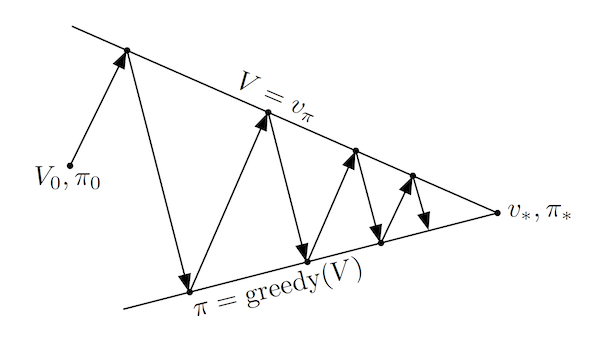
\includegraphics[width=12cm, height=8cm]{vf_policy_intersecting_lines.png}
\end{frame}

\begin{frame}
\frametitle{Generalized Policy Iteration (GPI)}
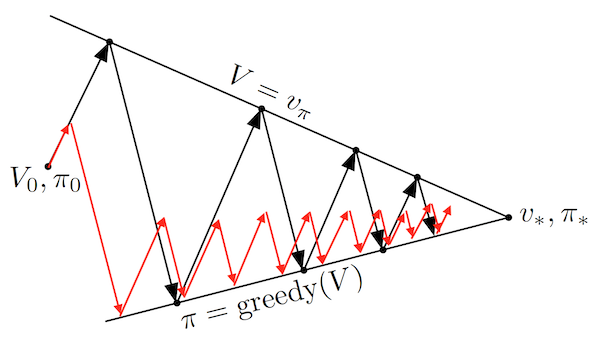
\includegraphics[width=12cm, height=8cm]{gpi.png}
\end{frame}

\begin{frame}
\frametitle{Value Iteration and Reinforcement Learning as GPI}
\pause
\begin{itemize}[<+->]
\item Value Iteration takes only one step of Policy Evaluation
$$\pi_1 = G(\bm{V_0}) \text{ : } \bm{V_0} \rightarrow \bm{B}^{\pi_1}(\bm{V_0}) = \bm{V_1}$$
$$\pi_2 = G(\bm{V_1}) \text{ : } \bm{V_1} \rightarrow \bm{B}^{\pi_2}(\bm{V_1}) = \bm{V_2}$$
$$\ldots$$
$$\ldots$$
$$\pi_{j+1} = G(\bm{V_j}) \text{ : } \bm{V_j} \rightarrow \bm{B}^{\pi_{j+1}}(\bm{V_j}) = \bvs$$
\item RL updates either a subset of states or just one state at a time
\item Large-scale RL updates function approximations of a VF
\item These can be thought of as {\em partial} Policy Evaluation/Improvement
\end{itemize}
\end{frame}

\begin{frame}
\frametitle{Asynchronous Dynamic Programming}
\pause
The DP algorithms we've covered are qualified as {\em Synchronous DP}:
\pause
\begin{itemize}
\item {\em All} states' values are updated in each iteration
\item "Simultaneous" state updates implemented by updating a copy of VF
\end{itemize}
\pause
{\em Asynchronous} DP can update subset of states, or update in any order
\pause
\begin{enumerate}[<+->]
\item {\em In-place} updates enable updated values to be used immediately
\item {\em Prioritized Sweeping} keeps states sorted by their Value Function {\em gaps}
$$\text{ Gaps } g(s) = |V(s) - \max_{a\in \mathcal{A}} \{ \mathcal{R}(s,a) + \gamma \cdot \sum_{s' \in \mathcal{N}} \mathcal{P}(s,a,s') \cdot V(s') \}|$$
But this requires us to know the reverse transitions to resort queue
\item {\em Real-Time Dynamic Programming (RTDP)} runs DP {\em while} the agent is experiencing real-time interaction with the environment
\begin{itemize}
\item A state is updated when it is visited during the real-time interaction
\item The choice of action is governed by real-time VF-extracted policy
\end{itemize}
\end{enumerate}
\end{frame}

\begin{frame}
\frametitle{Episodic MDPs with unique state visits}
\pause
\begin{itemize}[<+->]
\item A fairly common specialization of MDPs enables great tractability:
\begin{itemize}
\item All random sequences terminate within fixed time steps (episodic MDP)
\item A state is encountered at most once in an episode
\end{itemize}
\item This can be conceptualized as a \href{https://en.wikipedia.org/wiki/Directed_acyclic_graph}{\underline{\textcolor{blue}{Directed Acyclic Graph (DAG)}}}
\item Each node in the DAG is a (state, action) pair
\item Prediction/Control solved by ``backwards walk'' from terminal nodes
\item Bellman Equation enables simply {\em setting the VF} of a visited node
\item Avoids the expensive ``iterate to convergence'' method of classical DP
\item States visited (and VFs set) in order of reverse \href{https://en.wikipedia.org/wiki/Topological_sorting}{\underline{\textcolor{blue}{Topological Sort}}}
\item Next we cover a special case of DAG MDPs: finite-horizon MDPs
\end{itemize}
\end{frame}

\begin{frame}
\frametitle{Finite-Horizon MDPs}
\pause
\begin{itemize}[<+->]
\item Finite-Horizon Markov Decision Processes are characterized by:
\begin{itemize}
\item Each sequence terminates within a finite number of time steps $T$
\item Each time step has a separate (from other time steps) set of states
\end{itemize} 
\item Denote states at time $t$ as $\mathcal{S}_t$, terminal states as $\mathcal{T}_t$,  non-terminal states as $\mathcal{N}_t = \mathcal{S}_t - \mathcal{T}_t$ (note: $\mathcal{N}_T = \emptyset$), actions as $\mathcal{A}_t$, rewards as $\mathcal{D}_t$
\item Augment each state to include time-index: augmented state is $(t, s_t)$
$$\text{Entire MDP's States } \mathcal{S} = \{(t, s_t) | t = 0, 1, \ldots, T, s_t \in \mathcal{S}_t\}$$
\item Each $t$ gets its own state-reward transition probability function
$$(\mathcal{P}_R)_t: \mathcal{N}_t \times \mathcal{A}_t \times \mathcal{D}_{t+1} \times \mathcal{S}_{t+1} \rightarrow [0, 1]$$
\item Likewise, each $t$ gets its own policy $\pi_t: \mathcal{N}_t \times \mathcal{A}_t \rightarrow [0, 1]$
\item An overall policy $\pi: \mathcal{N} \times \mathcal{A} \rightarrow [0,1]$ composed of $(\pi_0, \pi_1, \ldots, \pi_{T-1})$
\end{itemize}
\end{frame}

\begin{frame}
\frametitle{Backward Induction for Finite MRP with Finite-Horizon}
\pause
\begin{itemize}[<+->]
\item VF for a given policy $\pi$ can be represented by time-sequenced VFs
$$V^{\pi}_t: \mathcal{N}_t \rightarrow \mathbb{R}$$
\item So Bellman Equation for $\pi$-implied Finite-Horizon MRP becomes:
$$V^{\pi}_t(s_t) = \sum_{s_{t+1} \in \mathcal{S}_{t+1}} \sum_{r_{t+1} \in \mathbb{D}_{t+1}} (\mathcal{P}_R^{\pi_t})_t(s_t, r_{t+1}, s_{t+1}) \cdot (r_{t+1} + \gamma \cdot V^{\pi}_{t+1}(s_{t+1}))$$
$$(\mathcal{P}_R^{\pi_t})_t(s_t, r_{t+1}, s_{t+1}) = \sum_{a_t \in \mathcal{A}_t} \pi_t(s_t, a_t) \cdot (\mathcal{P}_R)_t(s_t, a_t, r_{t+1}, s_{t+1})$$
\item ``Backward Induction'' algorithm for {\em finite MRP} with Finite-Horizon
\item Decrementing $t$ from $T$ to 0, and calculating $V_t^{\pi}$ from $V_{t+1}^{\pi}$
\item Running time is $O(m^2 T)$ where $|\mathcal{N}_t|$ is $O(m)$
\item $O(m^2 k T)$ to convert MDP to $\pi$-implied MRP ($|\mathcal{A}_t|$ is $O(k)$)
\end{itemize}
\end{frame}

\begin{frame}
\frametitle{Backward Induction for Finite MDP with Finite-Horizon}
\pause
\begin{itemize}[<+->]
\item Optimal VF $V^*$ can be represented by time-sequenced Optimal VFs
$$V^*_t: \mathcal{N}_t \rightarrow \mathbb{R}$$
\item So MDP Bellman Optimality Equation becomes: 
$$V^*_t(s_t) = \max_{a_t \in \mathcal{A}_t} \sum_{s_{t+1}} \sum_{r_{t+1}} (\mathcal{P}_R)_t(s_t, a_t, r_{t+1}, s_{t+1}) \cdot (r_{t+1} + \gamma \cdot V^*_{t+1}(s_{t+1}))$$
\item ``Backward Induction'' (Control) for {\em finite MDP} with Finite-Horizon
\item Decrementing $t$ from $T$ to 0, and calculating $V_t^*$ from $V_{t+1}^*$
\item (Associated) Optimal (Deterministic) Policy $(\pi^*_D)_t: \mathcal{N}_t \rightarrow \mathcal{A}_t$ is
$$(\pi^*_D)_t(s_t) = \argmax_{a_t \in \mathcal{A}_t} \sum_{s_{t+1}} \sum_{r_{t+1}} (\mathcal{P}_R)_t(s_t, a_t, r_{t+1}, s_{t+1}) \cdot (r_{t+1} + \gamma \cdot V^*_{t+1}(s_{t+1}))$$
\item Running time is $O(m^2 k T)$ where $|\mathcal{N}_t|$ is $O(m)$ and $|\mathcal{A}_t|$ is $O(k)$
\end{itemize}
\end{frame}

\begin{frame}
\frametitle{Dynamic Pricing for End-of-Life/End-of-Season}
\pause
\begin{itemize}[<+->]
\item Dynamic Pricing: Core to many businesses, flexing to supply/demand
\item We consider special case of products being sold at end of life/season
\item Assume we are $T$ days from season-end and our inventory is $M$ units
\item Assume no more incoming inventory during these final $T$ days
\item Set prices daily to max {\em Expected Total Sales Revenue} over $T$ days
\item Price for a given day picked from prices $P_1, P_2, \ldots, P_N \in \mathbb{R}$
\item Customer daily demand is $Poisson(\lambda_i)$ if Price $P_i$ is picked for the day
\item Note that demand can exceed inventory on any day, Sales $\leq$ Inventory
\end{itemize}
\end{frame}

\begin{frame}
\frametitle{Dynamic Pricing Model for End-of-Life/End-of-Season}
\pause
$$\mathcal{S}_t = \{(t, I_t) | I_t \in \mathbb{Z}, 0 \leq I_t \leq M\} \text{ for all } 0 \leq t \leq T$$
\pause
$$\mathcal{N}_t = \mathcal{S}_t \text{ and } \mathcal{A}_t = \{1, 2, \ldots, N\} \text{ for all } 0 \leq t < T, \text{ and } \mathcal{N}_T =\emptyset$$
\pause
$$I_0 = M \text{ and } I_{t+1} = \max(0, I_t - d_t) \text{ where } d_t \sim Poisson(\lambda_i) \text{ if } a_t = i$$
\pause
$$\text{Sales Revenue } \text{ on day } t \text{ is equal to } \min(I_t, d_t) \cdot P_t$$
\pause
$$
 (\mathcal{P}_R)_t(I_t, i, r_{t+1}, I_t - k) =
 \begin{cases}
 \frac {e^{-\lambda_i} \lambda_i^{k}} {k!} & \text{ if } k < I_t \text{ and } r_{t+1} = k \cdot P_i\\
 \sum_{j=I_t}^{\infty} \frac {e^{-\lambda_i} \lambda_i^{j}} {j!} & \text{ if } k = I_t \text{ and } r_{t+1} = k \cdot P_i\\
 0 & \text{ otherwise }
 \end{cases}
 $$
\end{frame}

\begin{frame}
\frametitle{Optimal Dynamic Pricing}
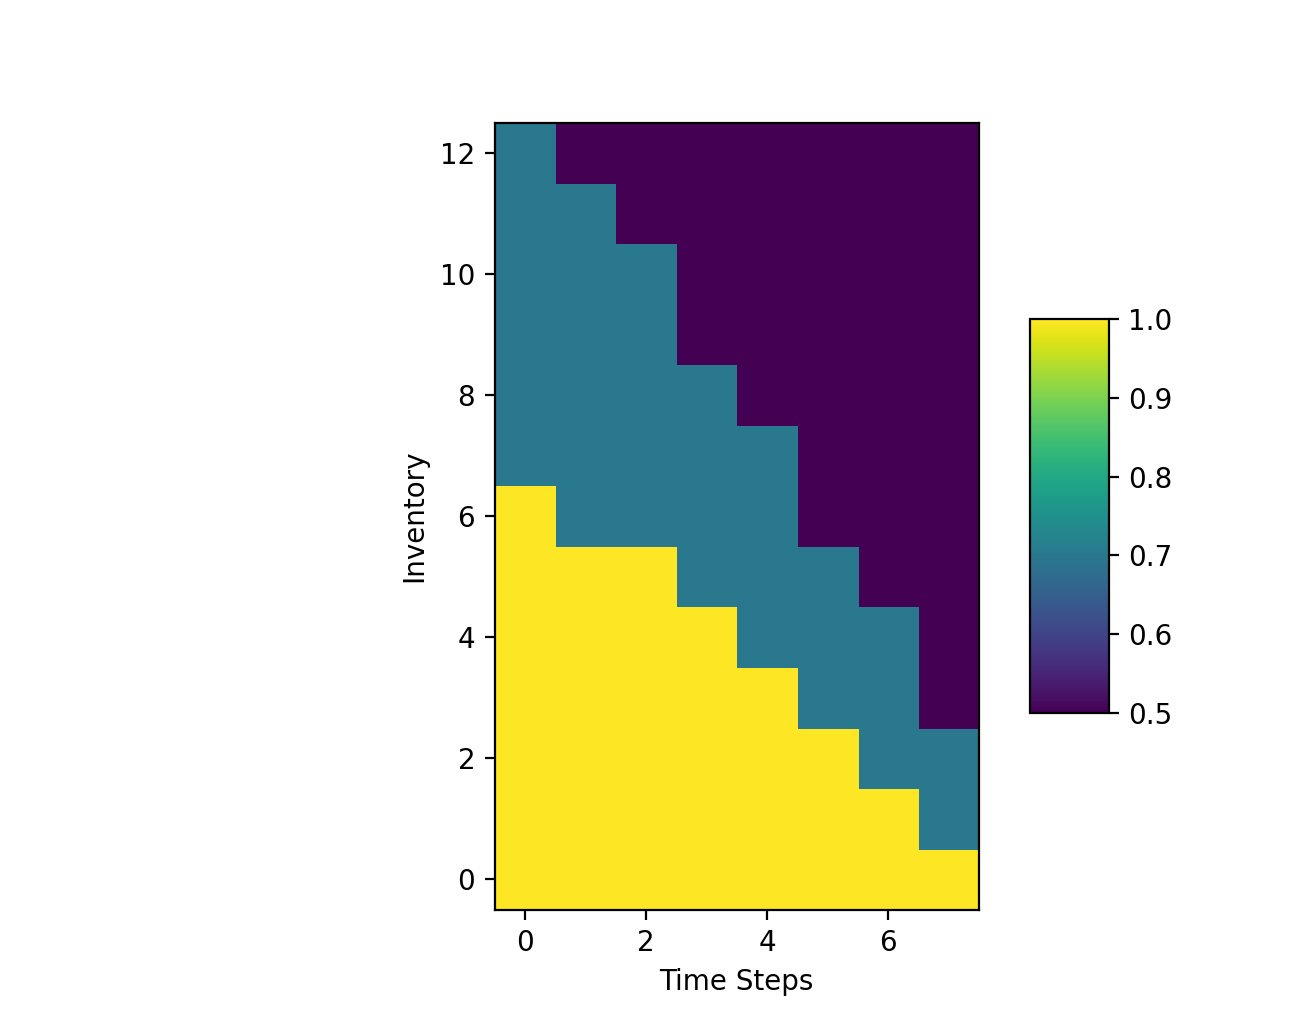
\includegraphics[width=12cm, height=8cm]{dynamic_pricing.png}
\end{frame}


\begin{frame}
\frametitle{Generalizations to Non-Tabular Algorithms}
\begin{itemize}[<+->]
\item Finite MDP algorithms we covered known as ``tabular'' algorithms
\item ``Tabular'' means MDP is specified as a finite data structure
\item More importantly, Value Function represented as a ``table''
\item These algorithms typically sweep through all states in each iteration
\item Cannot do this for large finite spaces or for infinite spaces
\item Requires us to generalize to function approximation of Value Function
\begin{itemize}[<+->]
\item Sample an appropriate subset of states 
\item Calculate the Value Function for those states (Bellman calculation)
\item Create/Update a func approx with the sampled states' calculated values
\end{itemize}
\item  The fundamental structure of the algorithms is still the same
\item Fundamental principles (Fixed-Point/Bellman Operators) still same
\item These generalizations known as {\em Approximate Dynamic Programming}
 \end{itemize}
\end{frame}


\begin{frame}
\frametitle{Key Takeaways from this Chapter}
\pause
\begin{itemize}[<+->]
\item Fixed-Point of Functions and Fixed-Point Theorem: Enables iterative algorithms to solve a variety of problems cast as Fixed-Point.
\item Generalized Policy Iteration: Powerful idea of alternating between {\em any} method for Policy Evaluation and {\em any} method for Policy Improvement, including methods that are partial applications of Policy Evaluation or Policy Improvement. This generalized perspective unifies almost all of the algorithms that solve MDP Control problems.
\item Backward Induction: A straightforward method to solve finite-horizon MDPs by simply walking backwards and {\em setting} the Value Function from the horizon-end to the start.
\end{itemize}
\end{frame}


\end{document}